% This is samplepaper.tex, a sample chapter demonstrating the
% LLNCS macro package for Springer Computer Science proceedings;
% Version 2.20 of 2017/10/04
%
\documentclass[runningheads]{llncs}
%
\usepackage{graphicx}
\usepackage{amsmath}
\usepackage{amssymb}
\usepackage[utf8]{inputenc} % Required for inputting international characters
\usepackage[T1]{fontenc} % Output font encoding for international characters
\usepackage[options ]{algorithm2e}
\usepackage{algorithm}% http://ctan.org/pkg/algorithm
%\usepackage{algpseudocode}% http://ctan.org/pkg/algorithmicx
\usepackage{mathpazo} % Use the Palatino font by default
\usepackage{array}% http://ctan.org/pkg/array
% Used for displaying a sample figure. If possible, figure files should
% be included in EPS format.
%
% If you use the hyperref package, please uncomment the following line
% to display URLs in blue roman font according to Springer's eBook style:
% \renewcommand\UrlFont{\color{blue}\rmfamily}

\begin{document}
%
\title{Impact of outliers and loss functions on XGBoost}

%Contribution Title\thanks{Supported by organization x.}}
%
%\titlerunning{Abbreviated paper title}
% If the paper title is too long for the running head, you can set
% an abbreviated paper title here
%
\author{Rao Kotagiri\inst{1}\orcidID{a} \and
Ziren\inst{1}\orcidID{b} \and
Prafull\inst{1}\orcidID{c}}
%
\authorrunning{F. Author et al.}
% First names are abbreviated in the running head.
% If there are more than two authors, 'et al.' is used.
%
\institute{The University of Melbourne}
%
\maketitle              % typeset the header of the contribution
%
\begin{abstract}
\paragraph{} The quantity of data we generate each day keeps on increasing. Today we are producing Exabytes of data per day, which is equal to the total data we had on earth in the year 2000. Various techniques are being used to utilize the data and gain knowledge from it. One such method is prediction modelling in machine learning. The accuracy of these models depends on multiple factors, of which one of the critical aspects is the presence of outliers. Outliers can induce additional loss, thus reducing the accuracy of prediction, and a small variation can sometimes lead to disastrous results. The two approaches in the proposal are based on outlier detection and outlier handling techniques. The first approach utilizes traditional outlier detection concepts like distance or similarity measure, cluster and spatial techniques for detecting and removing these outliers and thus making the predictions more accurate for machine learning algorithm called XGBoost. The second approach is based on the addition of user-defined loss functions, which are capable of making XGBoost model tolerable to outliers, thus lifting the requirement of removing the outliers. \\
\\


\keywords{Outlier Detection  \and Removal \and  Loss Function \and XGBoost.}
\end{abstract}
%
%
%
\section{Introduction}
\paragraph{} In most of the prediction tasks, we analyze a tremendous amount of data. If we want to generate accurate predictions, the initial step should be mitigating the effect of outliers on the model generation. This paper proposes two different techniques for handling outliers. Approach one combines an outlier detection framework to XGBoost prediction modelling process, to discover and eliminate outliers, thus making prediction modelling more accurate for XGBoost. The method uses outlier detection techniques based on properties like distance, time-series, ensemble etc. Using this technique, we can remove erroneous data as well as we might be able to identify the process which leads to the outlier generation. Process discovery leads to the implementation of outlier detection as various services like fraud detection, malicious node identification etc. 


% \paragraph{Prafull}The second approach is based on the addition of user-defined loss functions, which are capable of making XGBoost model tolerable to outliers, thus lifting the requirement of removing the outliers. In this approach, we penalize the outliers based on the domain requirement. For example, we want to make predictions for the right time to reach the airport to board a flight. What if we reach 45 minutes before or 5 minutes after the plane takes off? In both cases, there is a loss of time, but the magnitude of time alone does not justify the intensity of loss. Similarly, outliers can result in various types of loss, which can be tackled by using different user-defined loss functions.
\paragraph{} The second approach is based on the addition of user-defined loss functions, which are capable of making XGBoost model tolerable to outliers, thus lifting the requirement of removing the outliers. In this approach we construct a loss function which is less biased towards outliers than log loss (or other methods which have strong sensitivity to outliers) and has minor side effects on the normal points. The XGBoost has provided a couple of frequently used objective functions as a build-in parameter, such as logistic regression, squared loss and hinge loss \footnote{https://xgboost.readthedocs.io/en/latest/parameter.html}. However, only log squared error is sensitive to outliers and none of them uses architecture like Huber loss in those pre-defined functions, which could not meet our aim. Therefore, we customise the objective function to best fit the goal. The new function could have two choices based on the character of the point: (i) regular data are processed by a loss function which has less sensitivity to outliers (ii) whereas others are applied on outlier-sensitive loss function. One of challenges of this method is that outliers are difficult to be identified during training progress. A solution to that could be the use of unsupervised techniques from approach one, which does not require pro knowledge of outliers.
%A solution could be analysing the whole data using statistical methods before each time assigning a corresponding loss function.  Another solution could be identifying outliers after training.  Specifically, data are trained as the regular procedure firstly, then we can assume that a certain percentage of data which is ordered by evaluation methods are identified as outliers.  Thus, an ideally ’outlier-free’ dataset is obtained and could be used to train and test.



% we dont need this here...
\subsection{Application}
\paragraph{} Information about outlier can be extended in fields like finance, medical, etc. Some domain-specific implementation of outlier detection is as follows.

\paragraph{Intrusion Detection System: }There are applications which maintain data regarding a system call to the operating system, network logs, etc. Any abnormal data can lead us to a malicious event.
\paragraph{Credit-card fraud:} Credit card information like its number and security code at times is compromised. A particular credit card stores the patterns of shopping for a user, in case a user makes an unlikely purchase, the information can be treated and dealt as an outlier.
\paragraph{Environmental Sensors:} Devices are installed at strategic locations to monitor ecological behaviour. Any variation in the behaviour based on data points can be a possible event of interest.
\paragraph{Medical Diagnosis:} In medical, the data comes in many forms like images from MRI scans etc. An abnormal pattern in the image can be a disease.

%\subsection{Problem Statement}
%\paragraph{Prafull}How can we increase the accuracy of prediction for XGBoost? Alternatively, we can say that we are interested in finding reasons that induces inefficient behaviour in the machine learning algorithm and how can we tackle these problems. The question arises because we intend to gain knowledge from abundant data and make predictions. The predictions on real time event are quantified using loss functions. They map the event to a number which signifies the cost linked with that event. Our intention here is to investigate the performance of XGBoost model, for different user defined loss functions.

%\paragraph{Prafull} A useful outlier might lead us to a cure for disease or detection of fraud in the transaction, whereas most of the outliers are just useless data, generated by an erroneous process or wrong calculation. There are several ways of detecting outliers, some based on existing statistical methods like extreme value analysis, others explicitly designed for outlier detection like the isolation forest. In this paper, we propose an outlier detection framework that improves the accuracy of prediction for XGBoost by detecting and removing outliers. The outlier detection framework also intends to identify a threshold region as a percentage of data instance that can help us understand a trend with outlier detection.

% we dont need this here
%\paragraph{Ziren}We are provided a dataset which is split into two parts: training data $D_{train}$ and testing data $D_{test}$. The dataset consists of features $x_i^j = \{x_i^j | j = 1,2,3...n\}$ and corresponding response $y_i$ on $i^{th}$ data, where $n$ is the number of selected features. Each part of data may contain a small percentage $p$ of deviated points where $p \leq 5\%$. We use the training data to train the XGBoost model and the remaining data are used to test the performance of the model. The aim is identifying the outliers in the $D_{train}$ as much as possible and reducing side effects of those points on predicting results of $D_{test}$.

\subsection{Related Work}

% outlier detection methods

\paragraph{} A basic analogy of understanding outliers is in terms of local and global outliers. A global outlier is identified using a binary value of 0 and 1 whereas a local outlier is assigned a score based on the extent to which a point is an outlier. Usually, there is less prior known outliers. As a result, supervised learning methods are less effective in detection. Unsupervised learning methods, on the other hand, works well, as the methods are meant to deal with tasks with less prior information.

\paragraph{} The distribution of data can provide informative parameters,  which can be used for outlier detection. Such techniques are implemented on univariate datasets and are less effective., as the distribution parameters like mean, standard deviation are sensitive to outliers. 
Next in line is a metric based on depth, which stacks data point into arch layers. The point on the outer layer has a higher tendency to be an outlier. Less efficient for high dimensional data.

\paragraph{} The distance-based metric is also used to locate outliers. The technique utilizes the concepts of k nearest neighbours, where data points are ranked based on the distance with their neighbour. We then determine outliers by partitioning the data.  Finally, we also have K Nearest Neighbour and Local outlier factor-based techniques. Both the technoques utilizes concepts similar to density based approach.

% previous works on loss functions

% basic concept of XGBoost



% what is new loss function actually doing? reasons?

% consider mathematical expression in this section?

\section{Background}
\paragraph{} XGBoost is our baseline algorithm for anomaly detection and model performance. As a result, first section covers the historical development of Boosting and machine learning algorithms. The next section talks about the importance of removing irrelevant features, scaling data and choice of feature. The section also focus on how variation in data types impacts outlier detection. Followed by loss functions role in prediction modeling and outlier detection.The section contains a summary of gradient boosting techniques and a comparison of tree models with non-tree algorithms.


\subsection{XGBoost}
\paragraph{ }In 1998 Kearns and Valiant made a conjecture, which asked the question that is it possible to consolidate response from weak learners to form a strong learner. Robert Schapire paper on boosting algorithm was an answer to this conjecture. XGBoost is an implementation of gradient boosting by Friedman. The XGBoost is an greatly improved version of GBM. The main difference between XGBoost and GBM is that the definition of the objective functions. Moreover, the XGBoost additionally uses the complexity model in the objective function. From the perspective of Bias-variance trade-off, the complexity model can reduce the variance of the XGBoost model and prevent overfitting of that model.

%\paragraph{Ziren}The XGBoost is an greatly improved version of GBM. The main difference between XGBoost and GBM is that the definition of the objective functions. Specifically, the XGBoost produces an approximation to a prediction by expanding the equation using Taylor Expansion, which includes both first and second derivatives. Instead, the GBM only uses first derivative \citep{friedman2001greedy}. Moreover, the XGBoost additionally uses the complexity model in the objective function. From the perspective of Bias-variance trade-off, the complexity model can reduce the variance of the XGBoost model and prevent overfitting of that model. Secondly, in the implementation of the XGBoost, it refers column subsampling in random forest. This can reduce the computations and the overfitting. Thirdly, the parallelisation is available in the XGBoost package. It is implemented by sorting the data points before training and saving into a block structure. So in following computations, the algorithm will use the previous saved structure rather than recomputing, which makes parallelisation possible. This feature can be also benefited when large data are used. Overall, the XGBoost is generally much faster in computation efficiency based on features above.

\paragraph{} We will review the objective function of the XGBoost in the following paragraphs, as the loss function used in the objective function determines our second approach. The goal of XGBoost is building K regression trees that the expectation value is closing to the accurate value \citep{chen2016xgboost}. Assume there is a dataset which has $n$ observations with $x$ features each and with a corresponding variable $y$. We also define $\hat{y}_i$ as the prediction of each $y$, which can be shown as the result of applying a function on $x_i$
\begin{equation}
    \hat{y}_i = f(x_i)
\end{equation}
In the XGBoost, this function is the sum of $K$ trees on $i^{th}$ data $x_i$:
\begin{equation}
    f(x_i) = \sum^K_{k=1} f_k(x_i)
\end{equation}
where $f_k$ is calculating scores of $k^{th}$ tree using data $x_i$. An objective function can be represented as the sum of the loss function and the penalty of it:
\begin{equation}
    Obj = \sum^n_{i=1}l(y_i, \hat{y}) + \sum \Omega(f_k)
\end{equation}
where $l$ is the loss function and $\Omega$ is the regularisation which prevents large complexity of the objective function. Our are of interest lies with the loss function mentioned above in the objective function. How we can make the model more tolerable to outliers is explained in the next section.
%The term $\Omega$ in the XGBoost can be defined as 
%\begin{equation}
%    \Omega(f_k) = \gamma T + \frac{1}{2}\lambda||\omega||^2
%\end{equation}
%where $\gamma$ and $\lambda$ are $L_1$ and $L_2$ regularisation respectively, T is the number of leaves and $\omega$ is magnitude of leaf weights. This penalty part is one of differences to the general tree boosted algorithm, providing simpler and effective way to computer predictions. The prediction value at each $t^{th}$ step could be the current value add the value of $(t-1)^{th}$'s prediction

%\begin{equation}
%    \hat{y}^t_i = \sum^t_{k=1} f_k(x_i) = f_t(x_i) + \hat{y}_i^{t-1}
%\end{equation}
%Therefore, the corresponding objective function which selects the best tree at %$t^{th}$ step becomes
%\begin{equation}
%    Obj^t = \sum^n_{i=1}l(y_i, f_t(x_i) + \hat{y}_i^{t-1}) + \Omega(f_t) + %\text{constant}
%\end{equation}
%By applying Taylor expansion on the loss function $l$, this objective function could have the form as follow
%\begin{equation}\label{f:tylor-objective-function}
%    Obj^t = \sum^n_{i=1}[l(y_i,\hat{y}_i^{t-1}) + g_if_t(x_i) + %\frac{1}{2}h_if^2_t(x_i)] + \Omega(f_t) + \text{constant}
%\end{equation}
%where $g_i$ and $h_i$ are the first order and the second order derivative of the loss function applying data $x_i$. By replacing the regularisation part and simplification, we can write the objective value as
%\begin{equation}
%    Obj^t = \sum_{t=1}^T [(\sum g_i)\omega_j + \frac{1}{2}(\sum h_i + \lambda)\omega_j^2] + \gamma T
%\end{equation}
%We could assume that the regularisation parameter $\omega_j$ can be written as
%\begin{equation}\label{f:omega-j}
%    \omega_j^* = -\frac{G_j}{H_j + \lambda} 
%\end{equation}
%which is independent to the objective function. After further compression of the equation, we could have the best objective reduction
%\begin{equation}\label{f:final-objective-function}
%	Obj^*  =  -\frac{1}{2}\sum_{j=1}^T \frac{G_j^2}{H_j + \lambda} + \gamma T
%\end{equation}
%where the $G_j$ and the $H_j$ are defined as
%\begin{equation}
	%\begin{split}
		%G_j = & \sum_{i\in j}g_i\\
		%H_j = & \sum_{i\in j}h_i
	%\end{split}
%\end{equation}
%This objective function aims to measure how good a tree is \citep{chen2016xgboost}. In specific, the smaller the score is, the better the structure score of a tree is.

\subsection{Loss Functions}
\paragraph{}The choice of a loss function should reflect the discrepancy between predicted values and real values, which would be minimised. Based on the above equation, we can define any loss function in the XGBoost as long as the first and the second derivatives are provided. However, the choice of loss functions are difficult to be applied on various problems. Because we are analysing the regression loss functions, the classification loss function will be not considered.

\paragraph{} Least squared (LS) loss function is a popular and default loss function used in the regression. Disadvantage of using LS in the regression problems is that the LS loss function squares the error, hence in some circumstances the error largely affects the objective. For instance, since outliers typically have larger difference of predictions and observations, the errors would be magnified. As the result, a very bad score will be given to the outliers comparing with other outlier sensitive loss functions. There are many variant of the LS loss which eliminates some limitations from ordinary one. A study in have described an advanced version, Stagewise Least Square loss (SLS) function, which solves LS problem in each stage with updating a target variable, rather than using a single LS equation. It keeps the advantages from the raw function, such as simplicity and efficiency, and makes improvements like better scalability and robustness. Similarly, in, the Weight Least Square (WLS) loss function could minimise the loss function by adding a weight to each pair of the prediction and the observation.

\paragraph{}With the aim to minimise the error from heavy tailed points, the Huber loss is an algorithm that is more sensitive to outliers. It attends to minimise the error of outliers by setting up a different function to points which are greater than a threshold and also maintains high performance for normal errors. In, it mentioned that the least square loss performs faster running speed than the Huber loss, but the variance of the least square loss is bigger in the experiment.

\subsection{Traditional Outlier Detection}


\paragraph*{Feature Selection:} The choice and quality of features help in creating an accurate model. One of the experiment is conducted on the Twitter social network dataset, implementing outlier detection on Link Prediction Problem. The engineered features Jaccard Coefficient, Salton Cosine, AA are such efficient features that individual features can help to determine node outliers.
\paragraph*{Proximity Based:} We can describe a data point as a proximity-based outlier if the point lies in the sparse region, i.e. less populated area. Few simplified variations of proximity methods are a cluster, distance and density method. In Clustering and Density methods, the data is clustered/ grouped before outlier detection, and a new point is analysed as an outlier based on the distribution of pre-aggregated data. Whereas, in the distance-based method, the distance to the k nearest neighbour from the actual point is calculated. Proximity-based techniques are made in a way that they are capable of processing both noise and anomalies.
\paragraph*{Outlier Ensembles for High dimensional data:} Ensembling is the method in which the output from multiple learners is combined to give the final result. An Ensemble technique can combine classification, clustering and outlier detection etc. Ensemble method is essentially useful for high dimensional datasets where the properties of data vary with varying subspace.
\paragraph*{Outlier detection for Categorical and Timeseries data:} For Categorical Data the similarity between values can not be identified based on the distance or separation, and this creates a problem in the interpretation of such data. As a result, various domain oriented methods exist to handle categorical data, few of which are as follows. Extending the Linear model to categorical and mixed data, Proximity model for categorical data, Aggregate Statistical Similarity, The Contextual Similarity. In a time-series data, continuity and flow of time are robust. As the number of dimensions increases, this temporal continuity can weaken and lead to an anomaly.

\paragraph{Prafull} Although we have theoretical definitions for outliers, an accurate description of an outlier is based on the premises formed on data and the method adopted to deal with outliers. A generic version of the definition by Professor Hawkins is as follows. \textit{An outlier is an observation that deviates so much from other observations as to arouse suspicion that it was generated by a different mechanism.
} The applications of outlier detection are not limited to improving the model performance for a learner. 

%\subsection{Challenges in outlier detection}
%Outlier detection is one of the most critical aspects of machine learning, and it comes with many challenges, few of which are:

%\paragraph*{Modelling:} How we model non outlier and outlier data points dramatically determines the effectiveness of outlier detection. Distribution of data is a complicated factor in generating an efficient model, and so is the process of mapping data points into a statistical model. Few challenges in this area are, computational costs, parameter, hyper-parameter tuning.

%\paragraph*{Application requirements:} The domain of the problem determines the similarity index or unit of measure. This measure is then used to identify outliers. These measures keep changing with the requirement, and hence, it becomes impossible to determine generic or universal criteria for outlier detection. 

%\paragraph*{Noise:} Sometimes misunderstood as outlier, but noise and outliers are two different things. The presence of noise deforms the data, which sometimes makes the normal data appear as an outlier or might make an outlier look like a normal data point.

%\paragraph*{Comprehensibility :} If an outlier is a random error or an unexpected data point, we would like to remove it without analysing it, but if the outlier occurs in a medical trial, it can be of great importance. In case, the data point is an important outlier, the detection methodology must provide support to the findings. 

\section{Experimental Setup}
\subsection{Datasets and Source}

In evaluating each approach, we will use 5 datasets, which are listed below

\begin{enumerate}
    \item Experiment 1 \\
    Dataset: Link Prediction problem \\
    Source: Kaggle/ Twitter
    \item Experiment 2: \\
    Dataset: PJM Energy
    \item Experiment 4 \\
    Dataset: Spatial Dataset \\
    Source: UCI ML Repository
    \item Experiment 4\\
    House Sales in King County, USA
    \item Experiment 5 \\
    Medical Cost Personal \\
\end{enumerate}




\subsection{Architecture and Experiment Design}

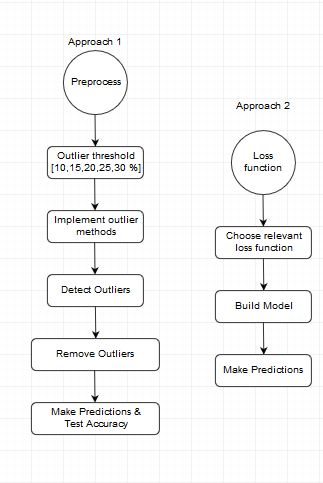
\includegraphics[scale=0.7]{arch.JPG}

\paragraph{Prafull Approach 1:} \\
\paragraph{Prafull} In the first approach, we have integrated an outlier detection framework with XGBoost, which efficiently finds and removes outliers. There are three different datasets used for method one. As we see above that the choice of feature influences the efficiency of an outlier detection process, we have generated features as and when required. Following this are the traditional machine learning steps involving removing the irrelevant features, one hot encoding where required and lastly scaling and transforming. Once the pre-processing of data is done, we implement the outlier detection framework, as seen in Algorithm 1 in the methodology section and also in the figure below. The system takes input of threshold(percentage of outliers to remove) and a dictionary containing all the detection techniques we want to execute and finally removes the outliers. The new dataset is then used to generate XGBoost model, which works more efficiently then the model created using the initial dataset. \\

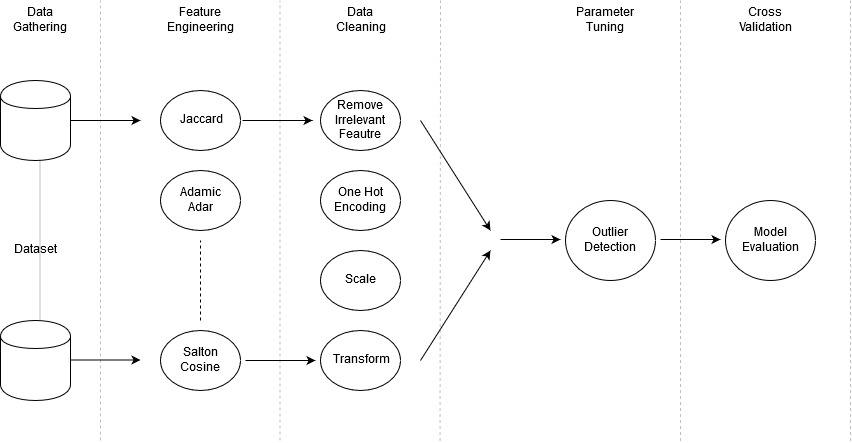
\includegraphics[scale=0.4]{hld-network.jpg}\par \\

% evaluation methods
\paragraph{Ziren Approach 2:}To evaluate the performance of a machine learning method in a regression problem, we often use distance as the standard metric. The meaning of distance in this case would be the error between the prediction and the real value
%\[d_i=y_i-\hat{y}_i\]
However, it is hard to compare the performance between different datasets using this method, because the range of differences in datasets may not be similar. Therefore, we can use the alternative method - the absolute relative difference of the error, which calculates the ratio of the residual and the actual value. 
%\begin{align}
    %d_i=y_i-\hat{y}_i \\
    %r_i = |\frac{y_i-\hat{y}_i}{y_i}| \\
    %min(R), Q_1(R), median(R), Q_3(R), max(R)
%\end{align}
In order to comparing the performance of our two methods, statistical method will be used. The most general approach of analysing a set of data statistically is using five number summary, which includes the minimum, first quartile, median, third quartile and maximum,
%\begin{equation}
    %min(R), Q_1(R), median(R), Q_3(R), max(R)
%\end{equation}
where $R$ is the collection of $r_i$ for all data in the dataset. These measurements describe 3 purposes of the dataset
\begin{itemize}
    \item Centre point of the distribution. 
    \item Spread of the distribution. This often refers to the variability of the data. 
    \item Shape of the distribution.
\end{itemize}

\section{Methodology}
%\paragraph{Prafull} As discussed above, there are two approaches for handling outliers. The first one is traditional approach of detecting and removing outliers for XGBoost, which we have referred as Prepossessing Approach. The second approach which makes XGBoost more tolerant to outliers is addressed as Loss function based approach.
\subsection{Approach 1: Outlier Detection and Processing}

The unique feature about the framework is that it does not require the user to run an experiment ten times in case he wants to detect outlier using ten different techniques on a single dataset. The methods start by taking in the input of the percentage of data points from the dataset, and we want to consider as outliers. The outlier fraction can be a list or a single value if it is a list the whole system works for all thresholds. The next step requires defining a dictionary of all the techniques we want to use on the dataset. Now, for one threshold and one detection technique, the system first assigns outlier score to all data points and then based on threshold it generates labels for a point being an outlier or not.

\begin{algorithm}[H]
\SetAlgoLined

 \STATE $t\gets threshold\_variations$
 
 %\STATE $columns\gets [useful columns]$ 
 
 \While{$t\neq empty$}{
  \STATE $outlier\_fraction\gets t.head(1)$
  
  \STATE $classifiers\gets \{ \\
     abod: angle\_based\_outlier\_detection \\
     cblof: cluseter\_based\_outlier\_detection \\
        ... \\
  \}$
  
  %\For{$name, $object \gets 1$ to $5$}    {
  \For{$cls\_name, $cls\_object in classifiers$ $}    {
      %\State {$instance$ $\gets$ {$instances$}}
      
       %\For{$k \gets 1$ to $5$}    {
       
          %\STATE $(col_a, col_b) \gets random.sample(population=columns, k=2)$
          
          \STATE $X\_train \gets dataset$ \\
          \STATE $cls\_object.fit(X\_train)$
          
          \STATE  $scores\_pred \gets cls\_object.decision\_function(X\_train)*-1$ \\
          \STATE $y\_pred \gets cls\_object.predict(X\_train)$
          
          \STATE $outliers \gets scores\_pred.head(outlier\_fraction)$
          
          \STATE $dataset\_new \gets X\_train.drop(outliers)$
          
          \STATE $result \gets crossValidate(dataset\_new, parameters)$
          
          \STATE $y\_pred \gets xgboost.predict(dataset\_new)$
       %}
   }                
   \EndFor
 }
 \caption{Outlier Detection}
\end{algorithm}



\subsection{Approach 2: Outlier Tolerable Loss Function (done)}

\paragraph{} The objective function can be customised in XGBoost by defining corresponding the first and second derivatives of a loss function. In this section, we will firstly consider a function that is not sensitive to outliers and another function which is outlier-sensitive. Then, a combination of previous two loss functions will be introduced, which is outlier-tolerable and also performs better.

\subsubsection{Square Loss and Log Square Loss}
The Square Loss is one of the most popular and basic loss function in the machine learning field. The idea is square the residual and generate first and second derivative.

%\[f(y-\hat{y}) = (y-\hat{y})^2\]
\begin{align}
  f(y-\hat{y}) = (y-\hat{y})^2 \\
  f'(y - \hat{y})= -2(y-\hat{y}) \\
  f''(y - \hat{y})= 2
\end{align}

%\begin{equation}
  %f''(y - \hat{y})= 2
%\end{equation}
The advantage of this function is that it can be applied on all real numbers without restrictions. However, it is too sensitive to outliers with large error and will generate large loss when processing those points. The Log Square Loss is a variation of the Log Loss, which applies an additional log on the error. The main purpose of this modification is alleviating the error and hence the influence of outliers with large error can be easily minimized. 

\begin{align}
	f(y - \hat{y}) = ln((y-\hat{y})^2) = 2ln(y-\hat{y}) \\
	gradient  = -\frac{2}{y - \hat{y}} \\
	hessian  = -\frac{2}{(y - \hat{y})^2}
\end{align}
%The first and the second derivatives are 
%\begin{equation}\label{5.1.2.1}
	%\begin{split}
		%gradient & = -\frac{2}{y - \hat{y}} \\
		%hessian & = -\frac{2}{(y - \hat{y})^2}
	%\end{split}
%\end{equation}

%However, there are two inappropriateness of this loss function. Firstly, the domain only accept positive numbers. It is worth mentioning that the first-order differentiation is not defined when the error $y-\hat{y}$ is non-positive and the second-order derivative cannot be applied by $(y-\hat{y}) = 0$. In the differentiation process we assumed the error will always be positive, because log function does not accept either negative numbers or zero. While in practice data, negative errors should be accepted. Secondly, the denominator of the training loss part should not always be negative. In specific, we may assume the denominator $H_j + \lambda$ is always negative, thus the training loss would be 0 or positive, according to the objective function. Therefore, the score of this tree structure is very likely to be a positive value. However, this may misguide the model to determine whether the tree is good, because the smaller value of a tree is better structure and in this case the better tree would have larger value. Apparently, this hessian will be always negative, in case of if $|\lambda|$ is smaller than $|H_j|$. Therefore, we need to modify the original derivatives to fit the XGBoost. We split the original function into 2 parts - values bigger or smaller than zero. The part with the error smaller than zero, an minus sign is applied before the equation. The detail expression of the function is expressed as follow:

However, there are two inappropriateness of this loss function. Firstly, the domain only accept positive numbers. It is worth mentioning that the first-order differentiation is not defined when the error $y-\hat{y}$ is non-positive and the second-order derivative cannot be applied by $(y-\hat{y}) = 0$. 

%We split the original function into 2 parts - values bigger or smaller than zero. The part with the error smaller than zero, an minus sign is applied before the equation. The detail expression of the function is expressed as follow:

%\begin{equation}
%  f(y - \hat{y})=\left\{
  %\begin{array}{@{}ll@{}}
    %2ln(y - \hat{y}), & (y - \hat{y}) > 0 \\
    %2ln(\hat{y} - y), & (y - \hat{y}) < 0
  %\end{array}\right.
%\end{equation}

%\begin{equation}
  %f'(y - \hat{y})=\left\{
  %\begin{array}{@{}ll@{}}
    %\frac{-2}{y - \hat{y}}, & (y - \hat{y}) > 0 \\
    %\frac{2}{\hat{y} - y} , & (y - \hat{y}) < 0
  %\end{array}\right.
%\end{equation}

%\begin{equation}
  %f''(y - \hat{y})=\left\{
  %%\begin{array}{@{}ll@{}}
    %\frac{2}{(y - \hat{y})^2}, & (y - \hat{y}) > 0 \\
    %\frac{2}{(\hat{y} - y)^2} , & (y - \hat{y}) < 0
  %\end{array}\right.
%\end{equation}
%It is obvious that both derivatives can be further simplified because they have the equivalent expressions. So equations are merged respectively and we obtain the final form of the modified Log Square Loss
%\begin{equation}
  %f'(y - \hat{y})= \frac{-2}{y-\hat{y}}, \text{when } y-\hat{y} \neq 0
%\end{equation}

%\begin{equation}
  %f''(y - \hat{y})= \frac{2}{(y - \hat{y})^2}, \text{when } y-\hat{y} \neq 0
%\end{equation}

%Finally, the value of when $y - \hat{y} = 0$ is assumed to be 0 in both derivatives, because of perfect prediction.

%\begin{equation}
  %f'(y - \hat{y})= 0, \text{when } y-\hat{y} = 0
%\end{equation}

%\begin{equation}
  %f''(y - \hat{y})= 0, \text{when } y-\hat{y} = 0
%\end{equation}

%There is a critical issue when we apply the Log Square Loss on the dataset with large magnitude, such as 1000000 and 2500000, that the Log Square Loss will produce constant predictions. The reason of this problem could be that the difference between each residual $y - \hat{y}$ would be similar when the residual is large, although the relative difference is small. For example, we assume that there are 2 predictions and real values such that $y$ = 1000000, 2500000 and $\hat{y}$ = 900000, 1000000 respectively, then residuals would be 100000 and 1500000, with relative difference 10\% and 60\% respectively. However, the Log Square Loss will generate results 23.02 for 10\% one and 28.44 for 60\% one by simply applying $log(error^2)$, which are very similar and will misguide the model to believe that both of results are good, whereas apparently the latter one should be classified as a bad prediction. Therefore, a suitable value of target variable should be selected. In the later evaluations, we will multiply a coefficient to make the mean of target variable around 10 if the mean value of it is significantly large, ensuring the best performance of the Log Square Loss.
\subsubsection{Mixed Loss} Based on the shortcomings and advantages of the above two loss function we propose a new function termed as Mixed Loss. % Previous sections described two loss functions which could be used to process different data. The Square Loss function is usually applied on data which have small errors because it will magnify the error of the outlier point, whereas the Log Square Loss is suitable for data with many outliers but it performs bad in normal points. In this section, we will show a loss function that combines those features.

The basic idea is splitting a loss function into 2 parts: if the error is less than a certain value, it uses the first function which is less sensitive to outliers to calculate the error; Otherwise, another function that is more sensitive to outliers will be applied. This can be expressed in a formula
\begin{equation}
  f(x)=\left\{
  \begin{array}{@{}ll@{}}
    f_1(x), & x<=\theta \\
    f_2(x), & \text{otherwise}
  \end{array}\right.
\end{equation}
The threshold value $\theta$ can be determined by using smaller value of the third quartile based on the final prediction results of $f_1$ and $f_2$
\begin{equation}
    min(Q_3(f_1(y, \hat{y})), Q_3(f_2(y, \hat{y})))
\end{equation}
In this paper, we define $f_1(x)$ and $f_2(x)$ as follows
\begin{equation}
  f(x)=\left\{
  \begin{array}{@{}ll@{}}
    \text{Square Loss}, & x<=\theta \\
    \text{Log Square Loss}, & \text{otherwise}
  \end{array}\right.
\end{equation}
Because this loss function cannot be differentiated directly, we may calculate final results using the gradient and the hessian from each of the loss function separately
\begin{equation}
  f'(y - \hat{y})=\left\{
  \begin{array}{@{}ll@{}}
    -2*(y - \hat{y}), &  (y - \hat{y})<=\theta \\
    -\frac{2}{y - \hat{y}}, & \text{otherwise}
  \end{array}\right.
\end{equation}

\begin{equation}
  f''(y - \hat{y})=\left\{
  \begin{array}{@{}ll@{}}
    2, & (y - \hat{y})<=\theta \\
    \frac{2}{(y - \hat{y})^2}, & \text{otherwise}
  \end{array}\right.
\end{equation}
However, if the Log Square Loss performs much better overall, for example, there is large difference between the mean error, we should consider a new function that has better performance and not sensitive to outliers to replace the Square Loss.

We expected that this loss function can have performance between $f_1$ and $f_2$ overall. Since $f_1$ will be applied on most of data points, the Mixed Loss will have similar performance as the $f_1$, except outliers. More importantly, the error from outliers should be lowered and smaller than $f_1$, which shows the tolerability of outliers.


\section{Outcomes}
\subsection{Approach 1:}
\paragraph{} In below-mentioned graphs, the y-axis represents loss values, and the x-axis represents the variation in the outlier fraction. The plot represents the change in the loss as we keep increasing the number of outliers to remove. A trend can be observed from the below-presented graphs.  As we increase the outlier fraction, the loss first decreases and after a certain threshold, the loss again starts growing. This is an outcome in favour of our experiments, which proves the point that first, we are able to find outliers correctly and later when all the outliers are removed the outlier detection techniques are considering useful information as outliers. This threshold can be claimed to be fixed as it varies with the quality of the data generating process. \\
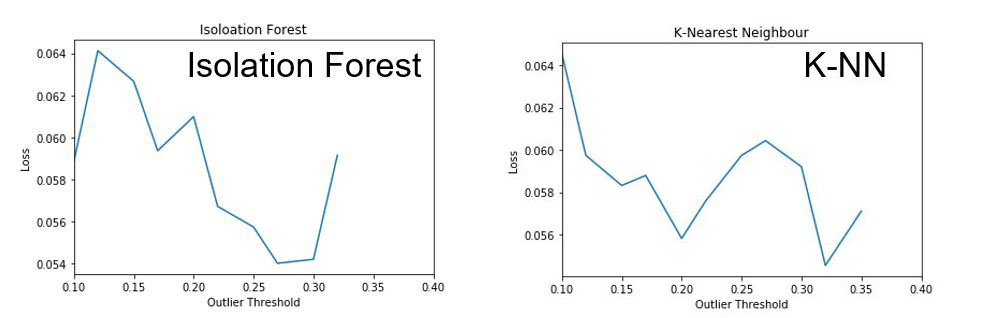
\includegraphics[scale=0.37]{tt2.jpg}

\subsection{Approach 2:}
\paragraph{}Tables below show five-number summary statistics of 3 loss functions described before applied on 5 datasets. Based on these summary statistics, we can see that the Mixed Loss performs as we expected. Specifically, (i) mid performance (ii) mid or lowest maximum (iii) similar to f1



\begin{table}[h]
\begin{center}
\begin{tabular}{|l|l|l|l|l|l|}
\hline
loss function & min & Q1 & median & Q3 & max \\ \hline
Least Square & 0.00004622 & 0.04750 & 0.1030 & 0.1909 & 3.607 \\ \hline
Log Square & 0.00005730 & 0.1258 & 0.2494 & 0.3671 & 4.330 \\ \hline
Mixed & 0.00004177 & 0.04656 & 0.1018 & 0.1871 & 2.667 \\ \hline
\end{tabular}
\end{center}
\caption{Summary Statistics of 3 Loss Functions Based On House Sales in King County, USA Dataset}\label{summary-statistics-3-functions-k3}
\end{table}


\begin{table}[h]
\begin{center}
\begin{tabular}{|l|l|l|l|l|l|}
\hline
loss function & min & Q1 & median & Q3 & max \\ \hline
Least Square & 0.00006899 & 0.06260 & 0.1328 & 0.2303 & 0.9222 \\ \hline
Log Square & 0.00007476 & 0.09142 & 0.1958 & 0.3308 & 1.074 \\ \hline
Mixed & 0.00004641 & 0.06521 & 0.1367 & 0.2350 & 0.8152 \\ \hline
\end{tabular}
\end{center}
\caption{Summary Statistics of 3 Loss Functions Based On Avocado Prices Dataset}\label{summary-statistics-3-functions-k1}
\end{table}


\subsection{Comparison}
\paragraph{Prafull} Feature bagging is highly effective in scenarios where a randomly selected feature is numerical, and the outliers can be straight away identified by higher values. The Angle based technique is more suitable for large size datasets as it does not require any complicated metric, just the variance in angles for similar points. Cluster-based methods perform exceptionally well for datasets which are clustered.

\section{Discussion}
\subsection{Strength of proposal}
\begin{itemize}
    \item Absorbing randomness of sampling: We have validated all the models and tests using ten-fold cross-validation, it has ensured that we have used all the instances in data, both as training and test set.
    \item The Increased accuracy of prediction:
    Approach 1 and 2 are able to deal with variations in the dataset and make the model either tolerable to outliers or improve the accuracy of prediction.
    \item Threshold Detection: The level of anomalies, removing which influenced the accuracy of prediction in a maximum number of cases lied between 15 to 30 per cent. Also, the trend explained above, which is first lowering then increasing of loss with an increase in threshold gives us the insight about the effectiveness of the technique.
    \item Overall, the Mixed Loss has been succeed to show achievement of our expectation. The tolerance of outliers is proved by use of Log Square Loss to process unusual points.
\end{itemize}


\subsection{Weakness of proposal}
\begin{itemize}
    \item The time complexity of techniques goes up to the square of the number of data instances multiplied by the number of features. Especially the ensemble technique which takes in multiple techniques as input give one average a better prediction accuracy, but is computationally expensive.
    \item Fair Evaluation and Benchmarks: If the outlier detected was not an actual outlier, but just an error in prediction can lead us to the loss of useful information. As a result, we require data analyst to manually test the outlier data instances. We did this work by gaining the domain knowledge and manually testing the data points.
    \item This loss function will be failed if the performance of the function $f_1$ that processing usual points is much worse than the Log Square Loss. In this case, the Log Square Loss will be always better and $f_1$ will be no longer necessarily needed. 
\end{itemize}

\section{Conclusion}
\paragraph{} The proposal utilizes two approaches to make better predictions. First, it uses traditional outlier detection techniques for removing outliers to improve XGBoost model performance. Secondly, the proposal uses user-defined loss functions to make the model tolerant of outliers.


\subsection{Future Work}
% Prafull's future work

% Ziren's future work
\paragraph{Ziren}For future directions and further improvements, we propose three key points. The first direction we propose is a new replacement function of the Least Square Loss should be considered, because it was not satisfied in two of our practical dataset tests. Specifically, it failed to achieve our expectation that non-outlier points were expected to be predicted with lower error than the Log Square Loss, whereas in testing Medical Cost Personal and Uniqlo StockPrice datasets, the error of normal points was higher than in the Log Square Loss. This replacement function should satisfy the following conditions: (i) it should be less sensitive to outliers (ii) it can accept all real numbers as the input (iii) it should be suitable for regression problems, instead of focusing on classifications (iv) the performance should be better than the Log Square Loss in predicting non-outliers. The second direction is to further improve the performance of XGBoost, input parameters such as number of maximum trees, maximum depth and learning rate can be optimised to best fit the objective function. We did not try to change those settings because our goal was to compare the performance of three loss functions and their tolerance to outliers in the same conditions. 




%
% the environments 'definition', 'lemma', 'proposition', 'corollary',
% 'remark', and 'example' are defined in the LLNCS documentclass as well.
%

%
% ---- Bibliography ----
%
% BibTeX users should specify bibliography style 'splncs04'.
% References will then be sorted and formatted in the correct style.
%
% \bibliographystyle{splncs04}
% \bibliography{mybibliography}
%

\end{document}
